\section{Demonstration of the Necessary Conditions for Catalyst Parameter Estimation \label{sec::necessary_cond}}

The catalyst mode detection algorithm presented fails when the catalyst is not saturated within the duration for a
significant length of time in the data. If the data-set does not have any regions of saturation, the approach fits
a saturated model as if the maximum achieved catalyst ammonia storage $(\max\lr{\sigma(k)})$ as the storage capacity of
the catalyst $(\Gamma)$. This is demonstrated using data from high-fidelity simulation model (AVL Cruise
\cite{AVLCruise}) tuned to RMC (Ramped Mode Cycle) test on a test-cell. The RMC test is then simulated with $\pm 20\%$
change in the gain of urea-dosing controller to change the length of the data where the catalyst remains saturated.
\begin{figure}[H]
        \centering
        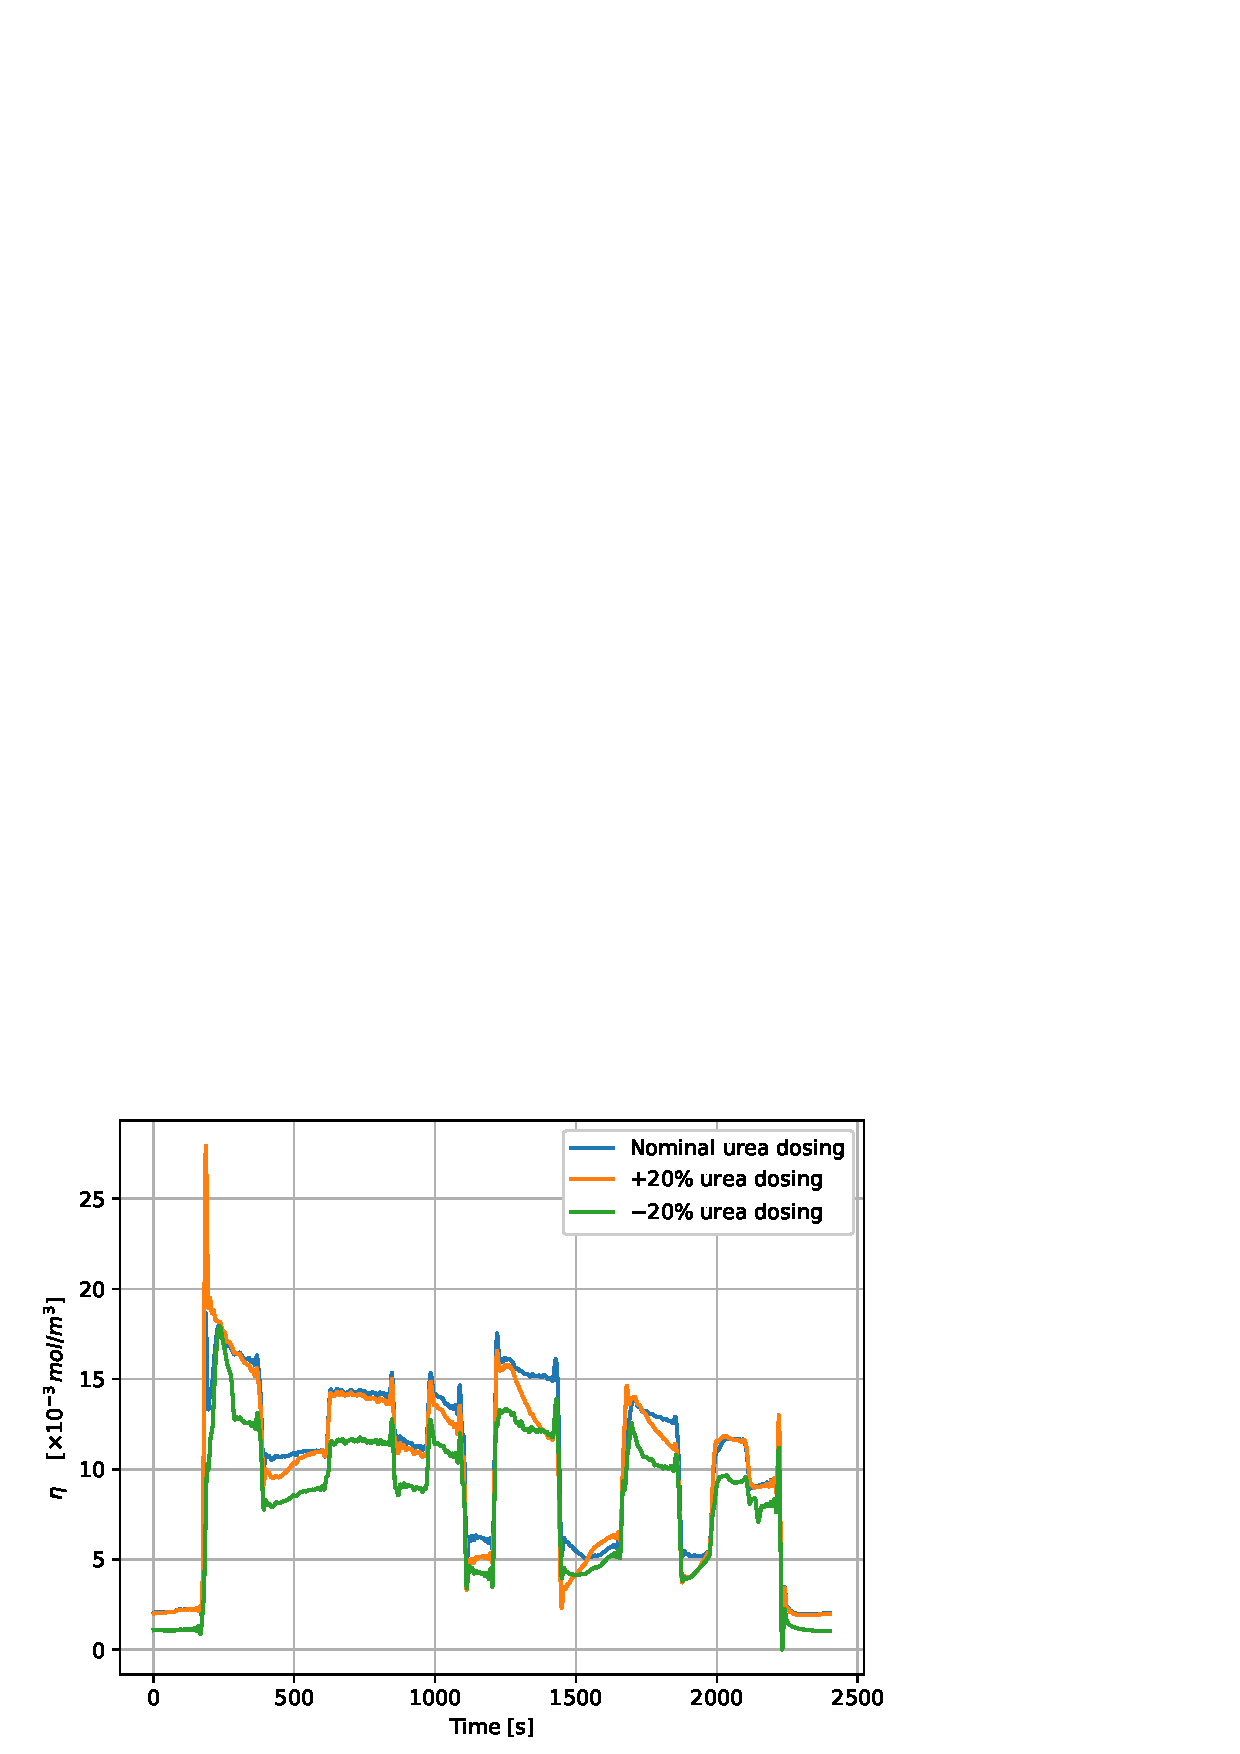
\includegraphics[width=\figWidth]{./figs/3_parm_ID/apx_necessary/eta_sim.png}
        \caption{RMC Test $NO_x$ Reduction with $\pm 20$ Urea Dosing Gain Variation}
        \label{fig::necessary_cond_sim}
\end{figure}
\begin{figure}[H]
        \centering
        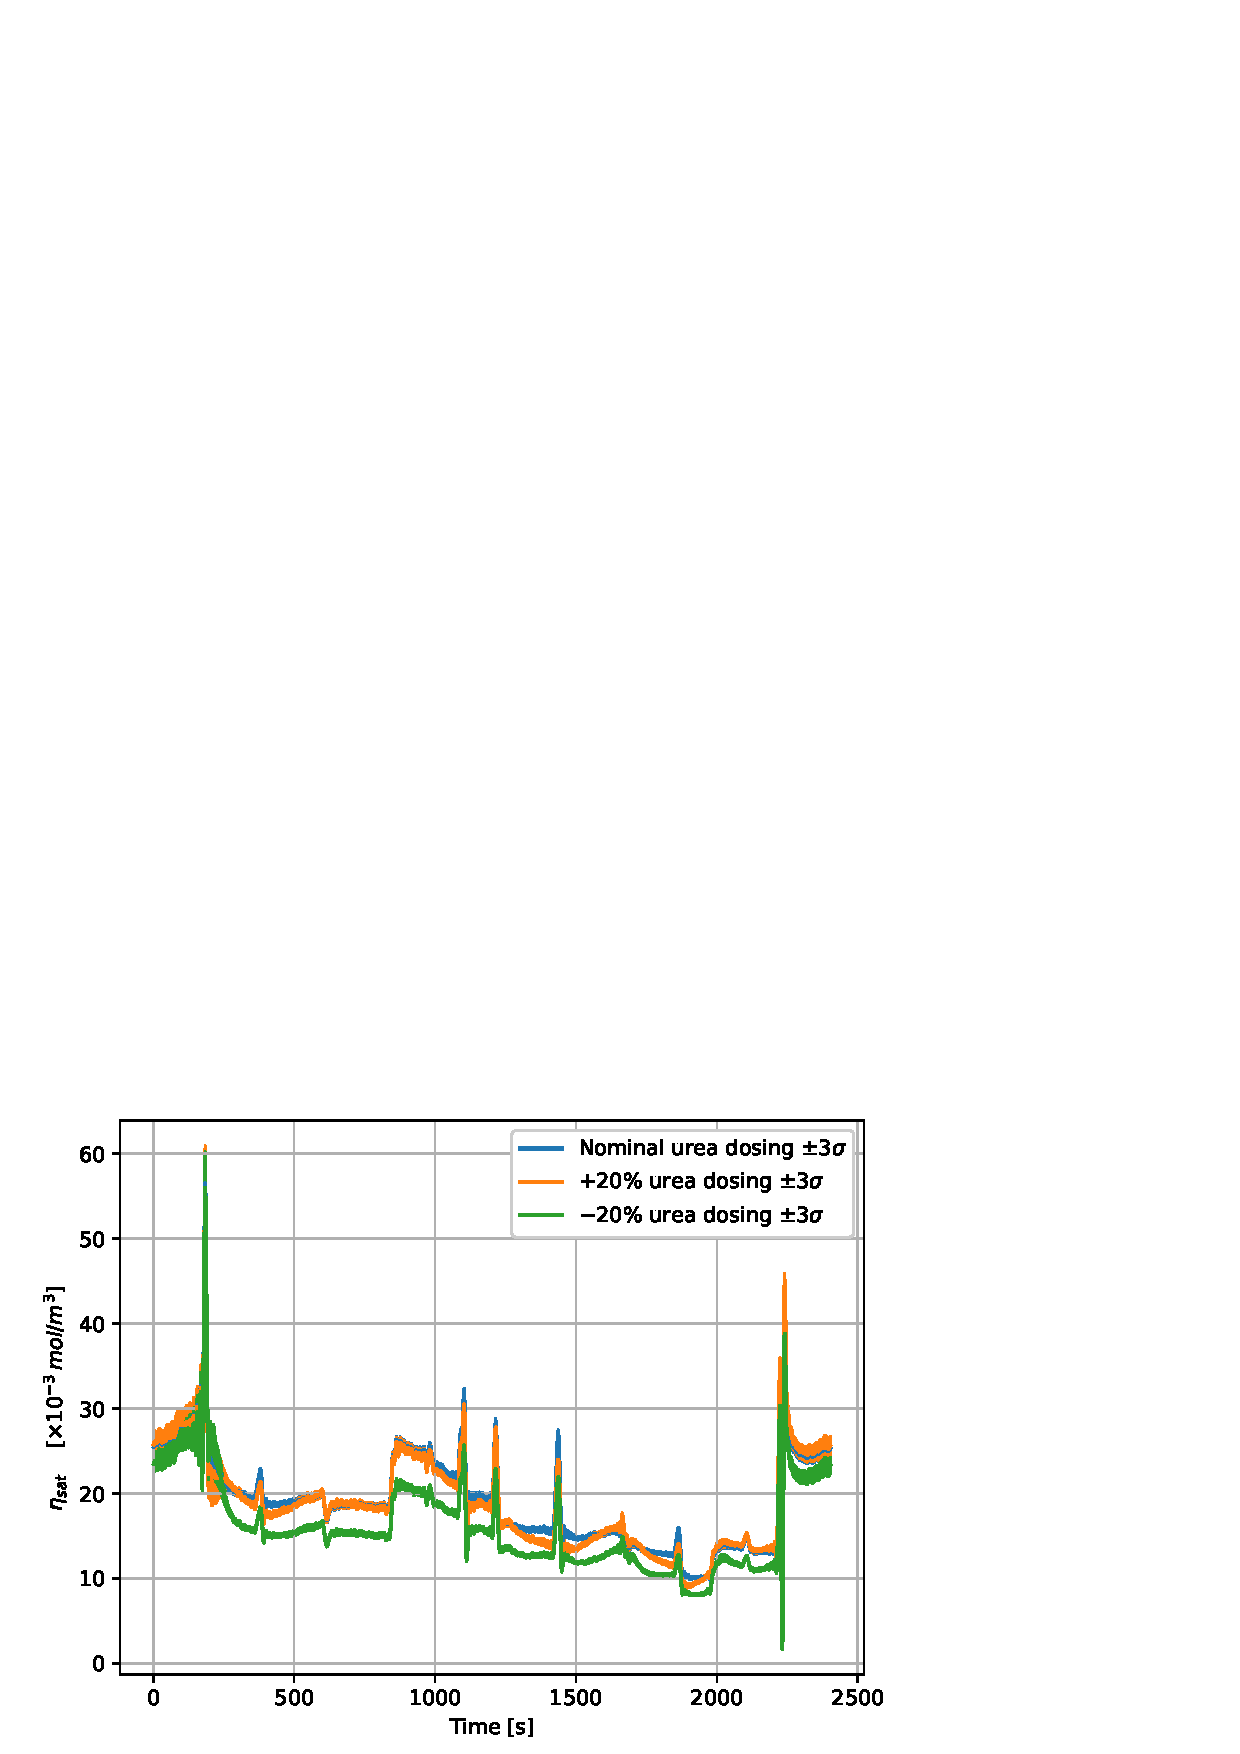
\includegraphics[width=\figWidth]{./figs/3_parm_ID/apx_necessary/eta_sat.png}
        \caption{Predicted $NO_x$ Reduction Under Catalyst Saturation}
        \label{fig::necessary_cond_sat}
\end{figure}
Figure-\ref{fig::necessary_cond_sim} shows no increase in $NO_x$ reduction when urea dosing is increased by $20\%$, which indicates that maximum $NO_x$ reduction is already reached at nominal urea dosing. This could be because the catalyst is saturated or because the inlet $NO_x$ concentration is sufficiently low. Conversely, a $20\%$ decrease in urea dosing decreases $NO_x$ reduction. When the $-20\%$ urea-dosing data are used to estimate saturated-model parameters, the model predicts a substantially lower $NO_x$ reduction under saturation than for the nominal and $+20\%$ dosing cases (Figure-\ref{fig::necessary_cond_sat}), the latter two giving essentially identical results.
